\chapter{Error Correcting Codes}
We can deliver messages all the way we want, but what if the message is lost, dropped, or corrupted? \\
In this chapter, we learn about error correcting codes: a major study of mathematics and EECS with many underlying theories and applications on media playback devices. If you have guessed from the combination of disciplines involved, these applications contain significant linear algebra based on finite fields!

\section{Erasure Errors}
Let us consider a corrupted message as follows:
\begin{ln-fig}{Erasure Error, Graphically Presented}{}
    \begin{center}
        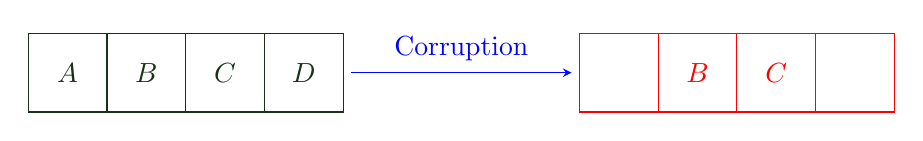
\begin{tikzpicture}
            \draw[green!10!black!90!]
                (0, 0) rectangle (1, 1)
                (0.5, 0.5) node{$A$}
                (1, 0) rectangle (2, 1)
                (1.5, 0.5) node{$B$}
                (2, 0) rectangle (3, 1)
                (2.5, 0.5) node{$C$}
                (3, 0) rectangle (4, 1)
                (3.5, 0.5) node{$D$};
            \draw[blue]
                [-stealth](4.1, 0.5) -- (6.9, 0.5);
            \draw[blue]
                (5.5, 0.8) node{Corruption};
            \draw[red]
                (7, 0) rectangle (8, 1)
                (7.5, 0.5) node{$\ $}
                (8, 0) rectangle (9, 1)
                (8.5, 0.5) node{$B$}
                (9, 0) rectangle (10, 1)
                (9.5, 0.5) node{$C$}
                (10, 0) rectangle (11, 1)
                (10.5, 0.5) node{$\ $};
        \end{tikzpicture}
    \end{center}
\end{ln-fig}
These errors are erasure errors, referring to the above situation(s) where a message with $n$ packets has lost at most $k$ packets during transmission. \\
To restore such messages, we can use some mathematical procedure. \\
Let us assume the contents of each packet is a number modulo $q$, where $q$ is prime. The properties over $GF(q)$ will then resolve the erasure error via polynomials. We are now applying note 8 contents! \\

Let us denote the message to be sent as $m_1, \dots, m_n$, where $m_i$ is a number in $GF(q)$. Then:
\begin{bindenum}
    \item[1.] There exists a unique polynomial $P(x)$ of degree $n - 1$ such that $P(i) = m_i$. Relevant properties were the focus subject of discussion in previous chapter.
    \item[2.] For each message to be sent, $m_i = P(i)$. We may then generate additional packets via evaluating this polynomial $P$ at points $n + k$. The interpolation would work fine as long as $n + k \leq q$, and thus we have attained a trasmitted codeword, which would have more packets than messages to account for packet loss.
    \item[3.] This polynomial $P(x)$ can be reconstructed from its values at any $n$ distinct points, since it is degree $n - 1$. Therefore, as long as $n$ packets are transmitted from the codeword, we can recover the original message. 
\end{bindenum}
So in summary, we'd transmit a $n + k$ packet codeword, which would have at most $k$ packages lost. However, the codeword is based on the original message, which has $n$ packets and thus is degree $n + 1$, and since we would have at least $n$ packets left after any errorneous transmission or disk-biting, disk-crushing, using my DVD as a frisbee... you get the point: at least $n$ packets are left for the polynomial interpolation to occur. \\
And the polynomial is characteristic of the message. As long as this polynomial can be retained from the successfully transmitted packets, we know the original message's individual packets via recovering the polynomial. \\
The uniqueness of our polynomial is thus CRUCIAL to the error correcting code!!!!!!!
\begin{ln-think}{Example of Recovering Erassure Errors}{}
    Let us review the example from lecture notes. Suppose our final result of transmission was something like this:
    \begin{center}
        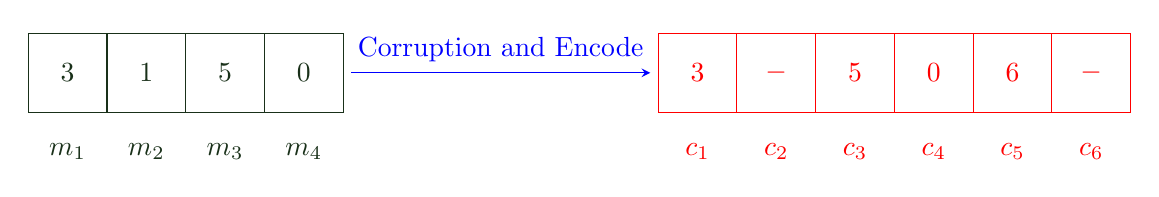
\begin{tikzpicture}
            \draw[green!10!black!90!]
                (0, 0) rectangle (1, 1)
                (0.5, -0.5) node{$m_1$}
                (0.5, 0.5) node{$3$}
                (1, 0) rectangle (2, 1)
                (1.5, -0.5) node{$m_2$}
                (1.5, 0.5) node{$1$}
                (2, 0) rectangle (3, 1)
                (2.5, -0.5) node{$m_3$}
                (2.5, 0.5) node{$5$}
                (3, 0) rectangle (4, 1)
                (3.5, -0.5) node{$m_4$}
                (3.5, 0.5) node{$0$};
            \draw[blue]
                [-stealth](4.1, 0.5) -- (7.9, 0.5);
            \draw[blue]
                (6, 0.8) node{Corruption and Encode};
            \draw[red]
                (8, 0) rectangle (9, 1)
                (8.5, -0.5) node{$c_1$}
                (8.5, 0.5) node{$3$}
                (9, 0) rectangle (10, 1)
                (9.5, -0.5) node{$c_2$}
                (9.5, 0.5) node{$-$}
                (10, 0) rectangle (11, 1)
                (10.5, -0.5) node{$c_3$}
                (10.5, 0.5) node{$5$}
                (11, 0) rectangle (12, 1)
                (11.5, -0.5) node{$c_4$}
                (11.5, 0.5) node{$0$}
                (12, 0) rectangle (13, 1)
                (12.5, -0.5) node{$c_5$}
                (12.5, 0.5) node{$6$}
                (13, 0) rectangle (14, 1)
                (13.5, -0.5) node{$c_6$}
                (13.5, 0.5) node{$-$};
        \end{tikzpicture}
    \end{center}
    The original message, notated as terms of $m$, will form a polynomial interpolation $P(x) = x^3 + 4x^2 + 5$. \\
    Therefore, the codeword would actually be a rectangular array of:
    \begin{center}
        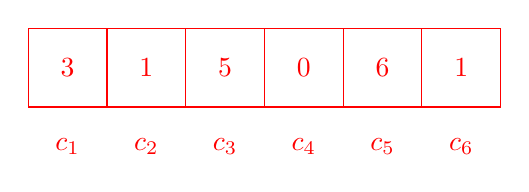
\begin{tikzpicture}
            \draw[red]
                (0, 0) rectangle (1, 1)
                (0.5, -0.5) node{$c_1$}
                (0.5, 0.5) node{$3$}
                (1, 0) rectangle (2, 1)
                (1.5, -0.5) node{$c_2$}
                (1.5, 0.5) node{$1$}
                (2, 0) rectangle (3, 1)
                (2.5, -0.5) node{$c_3$}
                (2.5, 0.5) node{$5$}
                (3, 0) rectangle (4, 1)
                (3.5, -0.5) node{$c_4$}
                (3.5, 0.5) node{$0$}
                (4, 0) rectangle (5, 1)
                (4.5, -0.5) node{$c_5$}
                (4.5, 0.5) node{$6$}
                (5, 0) rectangle (6, 1)
                (5.5, -0.5) node{$c_6$}
                (5.5, 0.5) node{$1$};
        \end{tikzpicture}
    \end{center}
    But, we are able to interpolate that exact polynomial $P(x)$ even if we are left with just $c_1, c_3, c_4, c_5$, since we have these $n$ points to interpolate a $n - 1$ degree polynomial. \\
    Therefore, computing $P(2)$ will recover $m_2$.
\end{ln-think}

\section{Polynomial Interpolation in Error Correction}
There are ways to perform polynomial interpolation other than the Lagrange Interpolation, which will be useful in the next section. \\
The goal of polynomial interpolation, again, is to take input of $d + 1$ pairs (points) and return a polynomial $p(x)$ such that it contains every point inputted. \\

\begin{ln-theorem}{Polynomial Interpolation for General Error}{}
    Let us disucss Polynomial Interpolation in this alternative method. \\
    We may first write a system of $d + 1$ linear equations in $d + 1$ variables, where the variables are the coefficients of the polynomial. \\
    Then, each equation is obtained by fixing $x$ to be one of $d + 1$ values (first item of per inputted tuple), with the rightside of equation (which is constant for a system solving context) be the second item of corresponding tuple. \\
    This polynomial interpolation method is fundamentally linear-algebra based, and only requires very fundamental skills (Gaussian Elimination) that we might just make it a new EECS 16A question.
\end{ln-theorem}

\section{General Errors}
The context of general error is, in summary, the general case of erasure errors. In this case, erased packets are replaced by corrupted packets, and our problem setting is once again, to work with a length-$n$ message with at most $k$ packets corrupted. \\
By the similarity of context, you may probably have guessed that our settings for solution once again follows these rules:
\begin{bindenum}
    \item Each character is a number modulo $q$ for some prime number $q$.
    \item We can describe a message as a polynomial $P(x)$ of degree $n - 1$ over $GF(q)$, such that each pair of message $(i, m_i)$ is contained by $P(x)$.
    \item To cope, with general errors specifically, we will transmit additional characters (so, sending a codeword, not a message).
\end{bindenum}
In this case, we transmit $2k$ additional characters. Therefore, at least $n + k$ of the received packets in a codeword is non-corrupted. \\
Now that we have the settings of our riddle, we must discuss: does Bob have sufficient information for recovering, or interpolating, the characteristic polynomial of original message? \\

First of all, for any $n + k$ packets of the codeword, there should exist a unique polynomial that fits all $n + k$ packets. So it is at least possible to recover the polynomial. \\
The proof of its uniqueness follows:
Among these $n + k$ points there can be at most $k$ errors. Let $P'(x)$ be another polynomial of degree $n - 1$ that goes through these $n + k$ packets, then at least $n$ of the packets would be contained by both $P$ and $P'$ However, our previous chapter has already revealed that a polynomial of degree $n - 1$ is defined by its values at $n$ points, so $P$ and $P'$ are in fact same polynomials. \\
Now that we know it is possible to find a polynomial, what is an efficient method of finding such polynomial, amidst the possible unlucky case of encountering some of the $k$ errors?
\begin{ln-theorem}{Error-Locator Polynomial}{}
    An error locator polynomial is designed to locate errors:
    \[E(x) = (x - e_1)(x - e_2)\dots(x - e_k)\]
    We do not know this polynomial explicitly, since we don't know where errors are. \\
    However, we have found that:
    \[P(i)E(i) = r_i E(i)\]
    where $r_i$ is the value of packet contained at index $i$ of the corrupted message. \\
    Since the value of $i$ has the constraint $1 \leq i \leq n + 2k$, we can indeed produce a system of $n + 2k$ linear equations with $n + 2k$ unknowns. \\

    Let us reflect on the approach. \\
    Define $Q(x) := P(x)E(x)$, which has degree $n + k - 1$ and therefore is described by $n + k$ coefficients. \\
    Meanwhile, $E(x)$ is described by $k + 1$ coefficients as a $k$-degree polynomial. \\
    Therefore, we interpolate $n + k$ coefficients from $Q(x) = r_x E(x)$ and $k$ coefficients from $E(x)$ (which is a polynomial of $(x - e_i)$, and we find that $e_i$ and there are $k$ of these). \\
    This forms $n + 2k$ linear equations for us to configure the coefficients of $Q(x)$ and $E(x)$. \\
    At last, we perform long division to acquire $P(x)$:
    \[P(x) = \frac{Q(x)}{E(x)}\]
\end{ln-theorem}
\begin{ln-theorem}{Correctness of Error-Locator Approach}{}
    Let us for the sake of proof assume the existence of alternative solutions $Q'$, $E'$, such that:
    \[P(x) = \frac{Q(x)}{E(x)} = \frac{Q'(x)}{E'(x)}\]
    Well, since we can follow from the definition of $Q$ to determine that $Q(x) = r_x E(x)$, we may conclude ahead:
    \[
        \begin{cases}
            Q'(x) = r_x E'(x) \\
            Q(x) = r_x E(x)
        \end{cases}
    \]
    Following the above equations:
    \begin{align*}
        Q'(x) E(x) &= r_x E(x) E'(x) \\
        Q(x) E'(x) &= r_x E(x) E'(x) \\
        Q'(x) E(x) &= Q(x) E'(x) \\
        \frac{Q(x)}{E(x)} &= \frac{Q'(x)}{E'(x)}
    \end{align*}
    Therefore, any possible set of polynomials would function to find us the right polynomial!
\end{ln-theorem}

\section{Personal Regard on This Topic}
It really probably is just about reading the notes a few more times and knowing how to perform polynomial interpolation :p \\
For now, there's nothing I'd like to add on top of the notes for this section.
